% !TEX program = xelatex
\documentclass[tikz, crop, border = {2pt 2pt 2pt 2pt}]{standalone}

\usepackage{concmath-otf}
\usetikzlibrary{calc, angles, quotes, patterns, decorations.pathreplacing, decorations.pathmorphing, calligraphy, arrows.meta}
\usetikzlibrary{math}
\usepackage{physics2}
\usepackage{derivative}
\usephysicsmodule{ab, ab.braket, ab.legacy, nabla.legacy, op.legacy}

\begin{document}
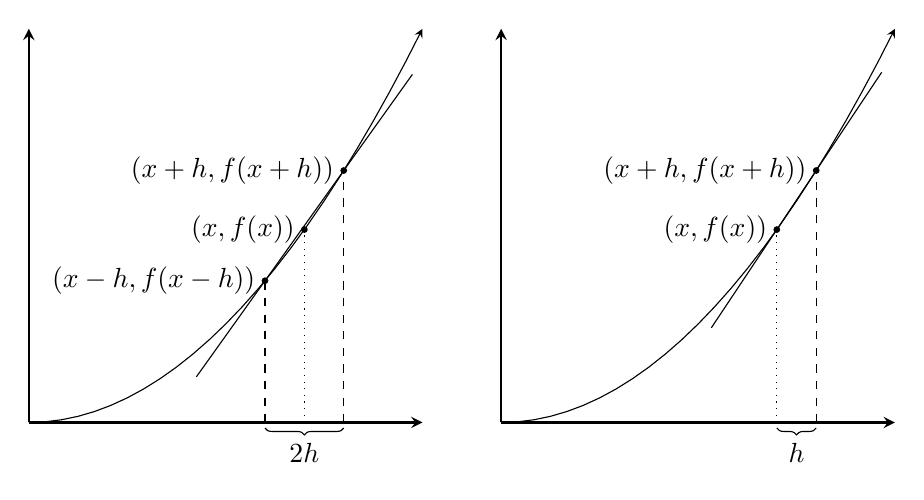
\begin{tikzpicture}
	\begin{scope}
		\draw[-stealth, thick] (0, 0) -- (5, 0);
		\draw[-stealth, thick] (0, 0) -- (0, 5);

		\def\h{0.5}
		\def\xz{3.5}

		\tikzmath{
			function f(\xz) {
					return (\xz*\xz/5);
				};
			\yz = f(\xz);
			\xhp = \xz + \h;
			\xhm = \xz - \h;
			\yhp = f(\xhp);
			\yhm = f(\xhm);
		}
		\draw[-stealth, domain = 0:5] plot (\x, \x*\x/5);
		\filldraw (\xhp, \yhp) circle (1pt) node[left] {\(\ab(x + h, f(x + h))\)};
		\filldraw (\xhm, \yhm) circle (1pt) node[left] {\(\ab(x - h, f(x - h))\)};
		\filldraw (\xz, \yz) node (x0) {} circle (1pt) node[left]{\(\ab(x, f(x))\)};

		\draw[dashed] (\xhp, 0) -- ++ (0, \yhp) node (xhm){};
		\draw[dashed] (\xhm, 0) -- ++ (0, \yhm) node (xhp){};

		\draw[dotted] (\xz, 0) -- ++ (0, \yz);

		\draw ($(xhm)!-1.5cm!(xhp)$) -- ($(xhp)!-1.5cm!(xhm)$);

		\draw[decorate, decoration = {brace, raise = 2pt, mirror}] (\xhm, 0) -- node[below = 4pt]{\(2h\)} (\xhp, 0);
	\end{scope}

	\begin{scope}[shift = {(6, 0)}]
		\draw[-stealth, thick] (0, 0) -- (5, 0);
		\draw[-stealth, thick] (0, 0) -- (0, 5);

		\def\h{0.5}
		\def\xz{3.5}

		\tikzmath{
			function f(\xz) {
					return (\xz*\xz/5);
				};
			\yz = f(\xz);
			\xhp = \xz + \h;
			\xhm = \xz - \h;
			\yhp = f(\xhp);
			\yhm = f(\xhm);
		}
		\draw[-stealth, domain = 0:5] plot (\x, \x*\x/5);
		\filldraw (\xhp, \yhp) circle (1pt) node[left] {\(\ab(x + h, f(x + h))\)};
		\filldraw (\xz, \yz) node (x0) {} circle (1pt) node[left]{\(\ab(x, f(x))\)};

		\draw[dashed] (\xhp, 0) -- ++ (0, \yhp) node (xhp){};

		\draw[dotted] (\xz, 0) -- ++ (0, \yz) node (x0){};

		\draw ($(x0)!-1.5cm!(xhp)$) -- ($(xhp)!-1.5cm!(x0)$);

		\draw[decorate, decoration = {brace, raise = 2pt, mirror}] (\xz, 0) -- node[below = 4pt]{\(h\)} (\xhp, 0);
	\end{scope}
\end{tikzpicture}
\end{document}
